% Options for packages loaded elsewhere
\PassOptionsToPackage{unicode}{hyperref}
\PassOptionsToPackage{hyphens}{url}
%
\documentclass[
  x11names]{article}
\usepackage{amsmath,amssymb}
\usepackage{lmodern}
\usepackage{iftex}
\ifPDFTeX
  \usepackage[T1]{fontenc}
  \usepackage[utf8]{inputenc}
  \usepackage{textcomp} % provide euro and other symbols
\else % if luatex or xetex
  \usepackage{unicode-math}
  \defaultfontfeatures{Scale=MatchLowercase}
  \defaultfontfeatures[\rmfamily]{Ligatures=TeX,Scale=1}
\fi
% Use upquote if available, for straight quotes in verbatim environments
\IfFileExists{upquote.sty}{\usepackage{upquote}}{}
\IfFileExists{microtype.sty}{% use microtype if available
  \usepackage[]{microtype}
  \UseMicrotypeSet[protrusion]{basicmath} % disable protrusion for tt fonts
}{}
\makeatletter
\@ifundefined{KOMAClassName}{% if non-KOMA class
  \IfFileExists{parskip.sty}{%
    \usepackage{parskip}
  }{% else
    \setlength{\parindent}{0pt}
    \setlength{\parskip}{6pt plus 2pt minus 1pt}}
}{% if KOMA class
  \KOMAoptions{parskip=half}}
\makeatother
\usepackage{xcolor}
\usepackage[margin=1in]{geometry}
\usepackage{graphicx}
\makeatletter
\def\maxwidth{\ifdim\Gin@nat@width>\linewidth\linewidth\else\Gin@nat@width\fi}
\def\maxheight{\ifdim\Gin@nat@height>\textheight\textheight\else\Gin@nat@height\fi}
\makeatother
% Scale images if necessary, so that they will not overflow the page
% margins by default, and it is still possible to overwrite the defaults
% using explicit options in \includegraphics[width, height, ...]{}
\setkeys{Gin}{width=\maxwidth,height=\maxheight,keepaspectratio}
% Set default figure placement to htbp
\makeatletter
\def\fps@figure{htbp}
\makeatother
\setlength{\emergencystretch}{3em} % prevent overfull lines
\providecommand{\tightlist}{%
  \setlength{\itemsep}{0pt}\setlength{\parskip}{0pt}}
\setcounter{secnumdepth}{-\maxdimen} % remove section numbering
\usepackage{fontspec} \usepackage{titling} \pretitle{\begin{center} \vspace{-3cm}
\includegraphics[width=\linewidth]{images/Base_info/logo.png}\LARGE\\} \posttitle{\end{center}} \usepackage{float} \usepackage{fancyhdr} \usepackage{ragged2e} \usepackage{caption} \usepackage{colortbl} \captionsetup[figure]{labelformat=empty} \arrayrulecolor{white} \pagestyle{fancy} \fancyhead[L,C]{} \fancypagestyle{plain}{\pagestyle{fancy}} \PassOptionsToPackage{dvipsnames,svgnames*,x11names*}{xcolor} \definecolor{ceil}{rgb}{0.57, 0.63, 0.81} \usepackage[export]{adjustbox} \usepackage{wrapfig} \usepackage{graphicx} \usepackage{caption}
\usepackage{booktabs}
\usepackage{longtable}
\usepackage{array}
\usepackage{multirow}
\usepackage{wrapfig}
\usepackage{float}
\usepackage{colortbl}
\usepackage{pdflscape}
\usepackage{tabu}
\usepackage{threeparttable}
\usepackage{threeparttablex}
\usepackage[normalem]{ulem}
\usepackage{makecell}
\usepackage{xcolor}
\ifLuaTeX
  \usepackage{selnolig}  % disable illegal ligatures
\fi
\IfFileExists{bookmark.sty}{\usepackage{bookmark}}{\usepackage{hyperref}}
\IfFileExists{xurl.sty}{\usepackage{xurl}}{} % add URL line breaks if available
\urlstyle{same} % disable monospaced font for URLs
\hypersetup{
  hidelinks,
  pdfcreator={LaTeX via pandoc}}

\author{}
\date{\vspace{-2.5em}Fecha de creación: 03 April, 2023}

\begin{document}

\setmainfont{Arial}
\setsansfont{Arial}
\setmonofont{Arial}

\newcommand\invisiblesection[1]{%
  \refstepcounter{section}%
  \addcontentsline{toc}{section}{\protect\numberline{\thesection}#1}%
  \sectionmark{#1}}

\fancyhead[R]{\textbf{http://doi.org/10.31687/SaremLR.19.181}}

%
  \refstepcounter{section}%
  \addcontentsline{toc}{section}{\protect\numberline{\thesection}GENERALIDADES}%
  \sectionmark{GENERALIDADES}
\vspace{-0.4cm}


\includegraphics[width=1\linewidth]{images/Base_info/logo}

\vspace{1cm}

\begin{minipage}{0.7\textwidth}
\vspace{0.3cm}
\fontsize{20}{24}\selectfont\textit{Pontoporia blainvillei}

\vspace{0.3cm}
\fontsize{30}{36}\selectfont Franciscana
\end{minipage}
\hspace{0.05\textwidth}
\begin{minipage}{0.25\textwidth}

\includegraphics[width=\textwidth]{images/vu.png}
\end{minipage}

\normalsize

\begin{figure}[H]

{\centering 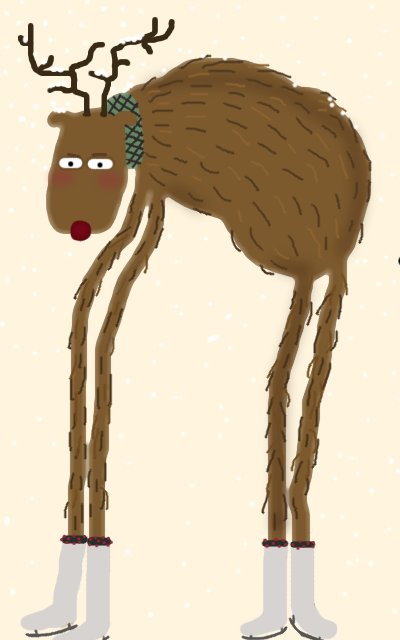
\includegraphics[width=0.35\linewidth]{photos/Blastocerus dichotomus} 

}

\caption{Fotos por Salvador Dali}\label{fig:image}
\end{figure}

\begin{center}\rule{0.5\linewidth}{0.5pt}\end{center}

\justifying

\textbf{Citar como:} Denuncio, Pablo E.; Paso Viola, Natalia ;
Cáceres-Saez, Iris; Cappozzo, H. Luis; Rodríguez, Diego; Mandiola,
Agustina. (2019). \emph{Pontoporia blainvillei}. En: SAyDS--SAREM (eds.)
Categorización 2019 de los mamíferos de Argentina según su riesgo de
extinción. Lista Roja de los mamíferos de Argentina.
\url{http://doi.org/10.31687/SaremLR.19.181}

\begin{center}\rule{0.5\linewidth}{0.5pt}\end{center}

\newpage

%
  \refstepcounter{section}%
  \addcontentsline{toc}{section}{\protect\numberline{\thesection}ÁREA DE DISTRIBUCIÓN ACTUAL}%
  \sectionmark{ÁREA DE DISTRIBUCIÓN ACTUAL}
\begin{table}[H]
\centering
\begin{tabular}[t]{>{\raggedright\arraybackslash}m{16cm}>{}m{16cm}}
\toprule
\cellcolor{ceil}{\textcolor{white}{\textbf{\rule{0pt}{14pt}ÁREA DE DISTRIBUCIÓN ACTUAL}}}\\
\bottomrule
\end{tabular}
\end{table}

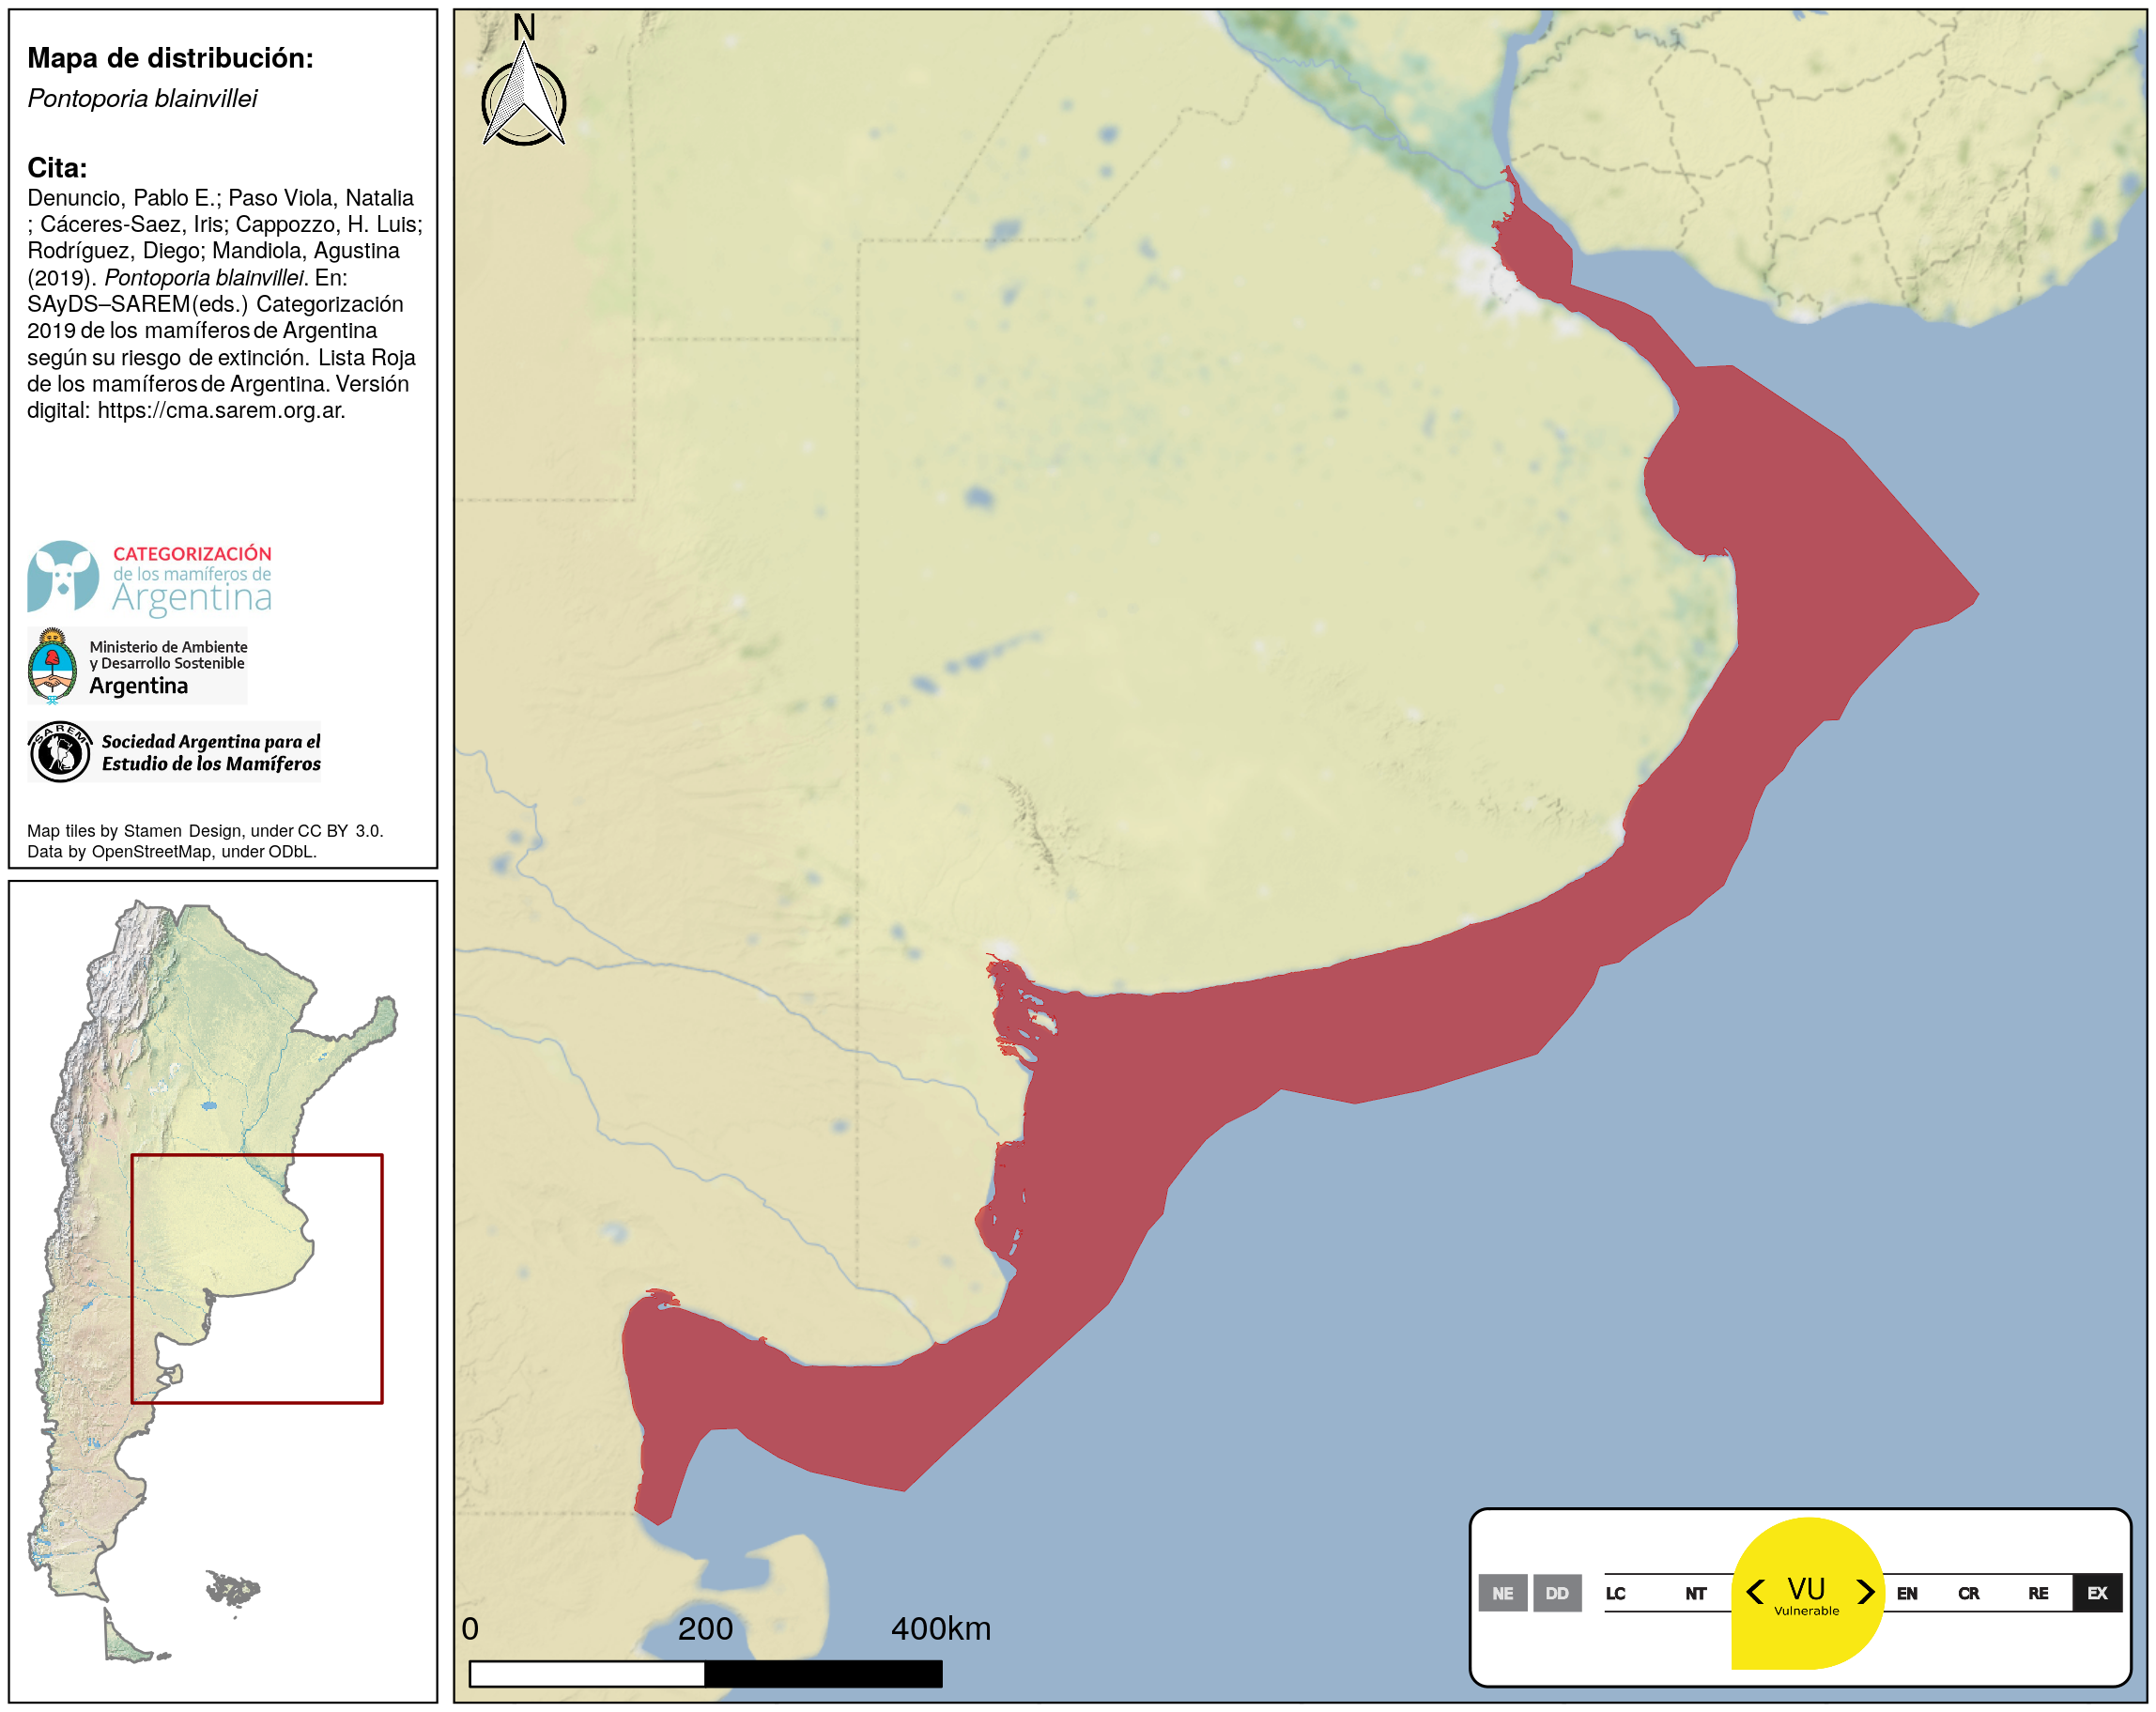
\includegraphics[width=1\linewidth]{maps/Cetartiodactyla/Pontoporia_blainvillei}

%
  \refstepcounter{section}%
  \addcontentsline{toc}{section}{\protect\numberline{\thesection}CATEGORÍAS DE CONSERVACIÓN}%
  \sectionmark{CATEGORÍAS DE CONSERVACIÓN}
\begin{table}[H]
\centering
\begin{tabular}[t]{>{\raggedright\arraybackslash}m{16cm}>{}m{16cm}}
\toprule
\cellcolor{ceil}{\textcolor{white}{\textbf{\rule{0pt}{14pt}CATEGORÍAS DE CONSERVACIÓN}}}\\
\bottomrule
\end{tabular}
\end{table}

\vspace{-0.4cm}

\textbf{Categoría Nacional de Conservación 2019}

VU (Vulnerable)

\textbf{Criterios y subcriterios}

A3cd

\textbf{Justificación de la categorización}

En los últimos 10 años se ha incrementado de forma exponencial la
información sobre la biología y la ecología del delfín franciscana en
Argentina, sin embargo, se carece de información actualizada sobre los
principales parámetros poblacionales para una evaluación de mayor
precisión sobre su estado de conservación. Estos parámetros son
principalmente estimaciones de mortalidad (últimos datos publicados
refieren a monitoreos realizados entre los años 2006--2009),
estimaciones de abundancia (últimos datos publicados refieren a
monitoreos realizados en los años 2003 y 2004) y tendencias
poblacionales. Sin embargo, y ante la continua evidencia de mortalidad
incidental directa (animales colectados por pescadores artesanales) e
indirecta (incrementos de varamientos vivos y muertos en la época de
mayor actividad pesquera) se presume que la situación de la especie
continúa siendo comprometida. Se evalúa a la especie en la categoría
Vulnerable (VU) debido a que se proyecta a futuro una reducción en el
tamaño poblaciona mayor al 30\% en las próximas 3 generaciones
(aproximadamente 50 años) (Criterio A3). Esta reducción afectará el área
de ocupación (AOO), la extensión de presencia (EOO) y la calidad del
hábitat (Subcriterio c). Asimismo hay datos de niveles de explotación
reales (captura incidental) (Subcriterio d). Se recomienda que~se llegue
a un consenso sobre el número de poblaciones dentro de la región
(también llamada Franciscana Management Área IV o FMA IV) y se tomen en
cuenta para realizar evaluaciones individuales en cada una de éstas, ya
que la evidencia demuestra que, tanto la mortalidad en redes de pesca
como la abundancia es heterogénea en todo el rango de su distribución en
aguas argentinas.

\textbf{Categoría Res. SAyDS 1030/04}

IC (Insuficientemente Conocida)

\textbf{Categorías nacionales de conservación previas (SAREM)}

\arrayrulecolor{white}

%
  \refstepcounter{section}%
  \addcontentsline{toc}{section}{\protect\numberline{\thesection}TAXONOMÍA Y NOMENCLATURA}%
  \sectionmark{TAXONOMÍA Y NOMENCLATURA}
\begin{table}[H]
\centering
\begin{tabular}[t]{>{\raggedright\arraybackslash}m{16cm}>{}m{16cm}}
\toprule
\cellcolor{ceil}{\textcolor{white}{\textbf{\rule{0pt}{14pt}TAXONOMÍA Y NOMENCLATURA}}}\\
\bottomrule
\end{tabular}
\end{table}

%
  \refstepcounter{section}%
  \addcontentsline{toc}{section}{\protect\numberline{\thesection}INFORMACIÓN RELEVANTE PARA LA EVALUACIÓN}%
  \sectionmark{INFORMACIÓN RELEVANTE PARA LA EVALUACIÓN}
\begin{table}[H]
\centering
\begin{tabular}[t]{>{\raggedright\arraybackslash}m{16cm}>{}m{16cm}}
\toprule
\cellcolor{ceil}{\textcolor{white}{\textbf{\rule{0pt}{14pt}INFORMACIÓN RELEVANTE PARA LA EVALUACIÓN}}}\\
\bottomrule
\end{tabular}
\end{table}

%
  \refstepcounter{section}%
  \addcontentsline{toc}{section}{\protect\numberline{\thesection}RANGO GEOGRÁFICO, OCURRENCIA Y ABUNDANCIA Y NOMENCLATURA}%
  \sectionmark{RANGO GEOGRÁFICO, OCURRENCIA Y ABUNDANCIA Y NOMENCLATURA}
\begin{table}[H]
\centering
\begin{tabular}[t]{>{\raggedright\arraybackslash}m{16cm}>{}m{16cm}}
\toprule
\cellcolor{ceil}{\textcolor{white}{\textbf{\rule{0pt}{14pt}RANGO GEOGRÁFICO, OCURRENCIA Y ABUNDANCIA Y NOMENCLATURA}}}\\
\bottomrule
\end{tabular}
\end{table}

%
  \refstepcounter{section}%
  \addcontentsline{toc}{section}{\protect\numberline{\thesection}DATOS MORFOMÉTRICOS}%
  \sectionmark{DATOS MORFOMÉTRICOS}
\begin{table}[H]
\centering
\begin{tabular}[t]{>{\raggedright\arraybackslash}m{16cm}>{}m{16cm}}
\toprule
\cellcolor{ceil}{\textcolor{white}{\textbf{\rule{0pt}{14pt}DATOS MORFOMÉTRICOS}}}\\
\bottomrule
\end{tabular}
\end{table}

%
  \refstepcounter{section}%
  \addcontentsline{toc}{section}{\protect\numberline{\thesection}RASGOS ETO-ECOLÓGICOS}%
  \sectionmark{RASGOS ETO-ECOLÓGICOS}
\begin{table}[H]
\centering
\begin{tabular}[t]{>{\raggedright\arraybackslash}m{16cm}>{}m{16cm}}
\toprule
\cellcolor{ceil}{\textcolor{white}{\textbf{\rule{0pt}{14pt}RASGOS ETO-ECOLÓGICOS}}}\\
\bottomrule
\end{tabular}
\end{table}

%
  \refstepcounter{section}%
  \addcontentsline{toc}{section}{\protect\numberline{\thesection}CONSERVACIÓN E INVESTIGACIÓN}%
  \sectionmark{CONSERVACIÓN E INVESTIGACIÓN}
\begin{table}[H]
\centering
\begin{tabular}[t]{>{\raggedright\arraybackslash}m{16cm}>{}m{16cm}}
\toprule
\cellcolor{ceil}{\textcolor{white}{\textbf{\rule{0pt}{14pt}CONSERVACIÓN E INVESTIGACIÓN}}}\\
\bottomrule
\end{tabular}
\end{table}

%
  \refstepcounter{section}%
  \addcontentsline{toc}{section}{\protect\numberline{\thesection}BIBLIOGRAFÍA}%
  \sectionmark{BIBLIOGRAFÍA}
\begin{table}[H]
\centering
\begin{tabular}[t]{>{\raggedright\arraybackslash}m{16cm}>{}m{16cm}}
\toprule
\cellcolor{ceil}{\textcolor{white}{\textbf{\rule{0pt}{14pt}BIBLIOGRAFÍA}}}\\
\bottomrule
\end{tabular}
\end{table}

\newpage

%
  \refstepcounter{section}%
  \addcontentsline{toc}{section}{\protect\numberline{\thesection}AUTORES}%
  \sectionmark{AUTORES}
\begin{table}[H]
\centering
\begin{tabular}[t]{>{\raggedright\arraybackslash}m{16cm}>{}m{16cm}}
\toprule
\cellcolor{ceil}{\textcolor{white}{\textbf{\rule{0pt}{14pt}AUTORES}}}\\
\bottomrule
\end{tabular}
\end{table}

\textbf{AUTORES}

\begin{tabu} to \linewidth {>{}l>{\raggedright\arraybackslash}p{2cm}>{\raggedright}X}
\toprule
\textbf{\cellcolor{gray!6}{Cáceres-Saez, Iris}} & \cellcolor{gray!6}{} & \cellcolor{gray!6}{Laboratorio de Ecología, Comportamiento y Mamíferos Marinos, División Mastozoología, Museo Argentino de Ciencias Naturales Bernardino Rivadavia (MACN-CONICET), CABA, Argentina}\\
\textbf{Cappozzo, H. Luis} &  & Museo Argentino de Ciencias Naturales Bernardino Rivadavia - CONICET, CABA, Argentina\\
\textbf{\cellcolor{gray!6}{Denuncio, Pablo E.}} & \cellcolor{gray!6}{} & \cellcolor{gray!6}{Instituto de Investigaciones Marinas y Costeras (IIMyC), Facultad de Ciencias Exactas y Naturales, Universidad Nacional de Mar del Plata-CONICET, Buenos Aires, Argentina}\\
\textbf{Mandiola, Agustina} &  & Instituto de Investigaciones Marinas y Costeras (IIMyC), Facultad de Ciencias Exactas y Naturales, Universidad Nacional de Mar del Plata-CONICET, Buenos Aires, Argentina\\
\textbf{\cellcolor{gray!6}{Paso Viola, Natalia}} & \cellcolor{gray!6}{} & \cellcolor{gray!6}{Laboratorio de Ecología y Conservación de Vida Silvestre, CADIC-CONICET, Ushuaia, Tierra del Fuego, Argentina}\\
\addlinespace
\textbf{Rodríguez, Diego} &  & Instituto de Investigaciones Marinas y Costeras (IIMyC), Facultad de Ciencias Exactas y Naturales, Universidad Nacional de Mar del Plata-CONICET, Buenos Aires, Argentina\\
\bottomrule
\end{tabu}

\textbf{COLABORADORES}

\begin{tabu} to \linewidth {>{}l>{\raggedright\arraybackslash}p{2cm}>{\raggedright}X}
\toprule
\textbf{\cellcolor{gray!6}{Cáceres, Manuel O.}} & \cellcolor{gray!6}{} & \cellcolor{gray!6}{Instituto Balseiro, Universidad Nacional de Cuyo y Centro Atómico Bariloche (CONAE), Bariloche, Río Negro, Argentina}\\
\textbf{Crespo, Enrique} &  & Laboratorio de Mamíferos Marinos, Centro para el Estudio de Sistemas Marinos, Centro Nacional Patagónico (CESIMAR - CENPAT – CONICET), Chubut, Argentina\\
\textbf{\cellcolor{gray!6}{Failla, Mauricio}} & \cellcolor{gray!6}{} & \cellcolor{gray!6}{Fundación Cethus, Vicente López, Buenos Aires, Argentina}\\
\textbf{García, Néstor A.} &  & Laboratorio de Mamíferos Marinos, Centro para el Estudio de Sistemas Marinos, Centro Nacional Patagónico (CESIMAR - CENPAT – CONICET), Chubut, Argentina\\
\textbf{\cellcolor{gray!6}{Gariboldi, María Constanza}} & \cellcolor{gray!6}{} & \cellcolor{gray!6}{Centro de Estudios Biomédicos, Biotecnológicos, Ambientales y Diagnóstico (CEBBAD), Universidad Mamimónides, CABA, Argentina}\\
\addlinespace
\textbf{Giardino, Gisela} &  & Instituto de Investigaciones Marinas y Costeras (IIMyC), Facultad de Ciencias Exactas y Naturales, Universidad Nacional de Mar del Plata-CONICET, Buenos Aires, Argentina\\
\textbf{\cellcolor{gray!6}{Panebianco, Victoria}} & \cellcolor{gray!6}{} & \cellcolor{gray!6}{Instituto de Investigación e Ingeniería Ambiental (3iA), Universidad Nacional de Gral. San Martín-CONICET, Buenos Aires, Argentina}\\
\textbf{Rodríguez Heredia, Sergio A.} &  & Fundación Mundo Marino, San Clemente del Tuyú, Buenos Aires, Argentina\\
\bottomrule
\end{tabu}

\end{document}
